\documentclass[
  11pt,
  letterpaper,
   addpoints,
   answers
  ]{exam}

\usepackage[utf8]{inputenc}
\usepackage{../exercise-preamble}
\usepackage{float}
\usepackage{subcaption}
\usepackage{pgfplots}
\pgfplotsset{compat=1.18}
% TikZ libraries needed for `right=.. of ..` and coordinate math
\usetikzlibrary{positioning,calc,arrows,arrows.meta}
% Alias de seguridad por si se escribe 'ikzstyle' por error
\let\ikzstyle\tikzstyle

\begin{document}

\noindent
\begin{minipage}{0.47\textwidth}

\includegraphics[width=\textwidth]{../fcfm_die}
\end{minipage}
\begin{minipage}{0.53\textwidth}
\begin{center} 
\large\textbf{Análisis de señales} (EL3203-2) \\
\large\textbf{Clase auxiliar 4} \\
\normalsize Prof.~Jorge Silva.\\
\normalsize Prof.~Aux.~Erik Sáez
\end{center}
\end{minipage}

\vspace{0.5cm}
\noindent
\vspace{.85cm}
\noindent
\begin{questions}

\question Encuentre la señal $x(n)$ si su transformada de Fourier a tiempo discreto está dada por

%----------------------------
\begin{figure}[H]
\centering
\begin{tikzpicture}[>=latex, line cap=round]

% ===== Parámetros editables =====
\def\wc{2.2}   % posición de ±\omega_c sobre el eje x
\def\halfW{0.4}% mitad del ancho de banda (W/2)
\def\H{2.0}    % altura de los rectángulos (amplitud)
% =================================

% Ejes
\draw[->] (-5,0) -- (5.5,0) node[below] {$\omega$};
\draw[->] (0,-0.2) -- (0,3) node[left] {$X(\omega)$};

% Marcas y etiquetas en x
\draw (-3.8,0.08) -- (-3.8,-0.08) node[below=2pt] {$-\pi$};
\draw ( 3.8,0.08) -- ( 3.8,-0.08) node[below=2pt] {$\pi$};
\draw (-\wc,0.08) -- (-\wc,-0.08) node[below=2pt] {$-\omega_c$};
\draw ( \wc,0.08) -- ( \wc,-0.08) node[below=2pt] {$\omega_c$};

% Marcas y etiquetas en y
\draw ( 0.08,1) -- (-0.08,1) node[left=2pt]  {$1$};
\draw ( 0.08,2) -- (-0.08,2) node[left=2pt]  {$2$};

% Rectángulo banda izquierda (centrado en -\omega_c)
\draw[line width=1.0pt]
  (-\wc-\halfW,0) -- (-\wc-\halfW,\H) -- (-\wc+\halfW,\H) -- (-\wc+\halfW,0);

% Rectángulo banda derecha (centrado en +\omega_c)
\draw[line width=1.0pt]
  (\wc-\halfW,0) -- (\wc-\halfW,\H) -- (\wc+\halfW,\H) -- (\wc+\halfW,0);

% Llave que indica el ancho W sobre la banda derecha
\draw[decorate, decoration={brace, amplitude=4pt}]
  (\wc-\halfW,\H+0.3) -- (\wc+\halfW,\H+0.3)
  node[midway, above=6pt] {$W$};

\end{tikzpicture}
\caption{Transformada de Fourier a tiempo discreto $X(\omega)$ de la señal $x(n)$.}
\end{figure}
Ahora considere una transformada de Fourier que en el rango $\left] -\frac{\pi}{2}, \frac{\pi}{2} \right]$ viene dado por:
\begin{align}
  X(\omega)= -\omega^{2} + \frac{\pi^{2}}{4}
\end{align}
bosqueje esta transformada y obtenga la señal en tiempo discreto asociada.
%----------------------------
\begin{solution}

\subsection*{Resolución 1.1}
 Para encontrar la señal $x(n)$ a partir de su transformada de Fourier a tiempo discreto $X(\omega)$, utilizamos la transformada inversa. Este procedimiento consiste en aplicar la integral inversa de la DTFT, que permite reconstruir la señal en el dominio temporal a partir de su representación espectral. A continuación, se presenta el planteamiento general, luego la DTFT inversa es
\[
x(n)=\frac{1}{2\pi}\int_{-\pi}^{\pi}X(\omega)\,e^{j\omega n}\,d\omega.
\]
Del gráfico, $X(\omega)=2$ sólo en los intervalos
\[
\left[-\omega_c-\frac{W}{2},\, -\omega_c+\frac{W}{2}\right]
\quad\text{y}\quad
\left[\omega_c-\frac{W}{2},\, \omega_c+\frac{W}{2}\right],
\]
y $X(\omega)=0$ fuera de ellos. Por lo tanto,
\begin{align*}
x(n)
&=\frac{1}{2\pi}\int_{-\omega_c-\frac{W}{2}}^{-\omega_c+\frac{W}{2}}2\,e^{j\omega n}\,d\omega
+\frac{1}{2\pi}\int_{\omega_c-\frac{W}{2}}^{\omega_c+\frac{W}{2}}2\,e^{j\omega n}\,d\omega. \tag{$\star$}
\label{star}
\end{align*}
Luego analizaremos dos casos de interes: $n\neq 0$ y $n=0$.
\begin{itemize}
  \item  \textbf{Cálculo para $n\neq 0$.} Cada integral es elemental:
\[
\int e^{j\omega n}\,d\omega=\frac{e^{j\omega n}}{j n}.
\]
Aplicando a \eqref{star}:
\begin{align*}
x(n)
&=\frac{1}{\pi}\left[\frac{e^{j\omega n}}{j n}\right]_{-\omega_c-\frac{W}{2}}^{-\omega_c+\frac{W}{2}}
+\frac{1}{\pi}\left[\frac{e^{j\omega n}}{j n}\right]_{\omega_c-\frac{W}{2}}^{\omega_c+\frac{W}{2}}\\[2mm]
&=\frac{1}{\pi j n}\Big(
e^{j n(-\omega_c+\frac{W}{2})}-e^{j n(-\omega_c-\frac{W}{2})}
+e^{j n(\omega_c+\frac{W}{2})}-e^{j n(\omega_c-\frac{W}{2})}
\Big)\\[1mm]
&=\frac{1}{\pi j n}\Big(
e^{-j n\omega_c}\big(e^{j n\frac{W}{2}}-e^{-j n\frac{W}{2}}\big)
+e^{+j n\omega_c}\big(e^{j n\frac{W}{2}}-e^{-j n\frac{W}{2}}\big)
\Big)\\[1mm]
&=\frac{1}{\pi j n}\,\underbrace{\big(e^{j n\frac{W}{2}}-e^{-j n\frac{W}{2}}\big)}_{=\,2j\sin(\frac{nW}{2})}\,
\underbrace{\big(e^{j n\omega_c}+e^{-j n\omega_c}\big)}_{=\,2\cos(n\omega_c)}\\[1mm]
&=\boxed{\,x(n)=\dfrac{4}{\pi n}\,\sin\!\Big(\frac{nW}{2}\Big)\cos(n\omega_c)\,},\qquad n\neq 0.
\end{align*}
Donde se han utilizado las identidades de euler y la definición de la función seno y coseno en términos de exponenciales complejas, las cuales son:
\begin{align}
\sin(x)&=\frac{e^{jx}-e^{-jx}}{2j},\\
\cos(x)&=\frac{e^{jx}+e^{-jx}}{2}.
\end{align}
\item \textbf{Caso $n=0$.} Usando directamente el área del espectro:
\[
\begin{aligned}
  x(0) &= \frac{1}{2\pi} \int_{-\omega_c-\frac{W}{2}}^{-\omega_c+\frac{W}{2}} 2\,d\omega
         + \frac{1}{2\pi} \int_{\omega_c-\frac{W}{2}}^{\omega_c+\frac{W}{2}} 2\,d\omega \\
       &= \frac{1}{2\pi} \left[ 2 \cdot \left( \left(-\omega_c+\frac{W}{2}\right) - \left(-\omega_c-\frac{W}{2}\right) \right)
         + 2 \cdot \left( \left(\omega_c+\frac{W}{2}\right) - \left(\omega_c-\frac{W}{2}\right) \right) \right] \\
       &= \frac{1}{2\pi} \left[ 2 \cdot (W) + 2 \cdot (W) \right] \\
       &= \frac{1}{2\pi} (4W) \\
       &= \frac{2W}{\pi}
\end{aligned}
\]
Es decir, $x(0)$ corresponde al área total bajo el espectro $X(\omega)$, que es la suma de las áreas de los dos rectángulos de altura $2$ y ancho $W$ cada uno.
\end{itemize}
Con lo que finalmente se tendra la funcion discreta sera:
\[
x(n)=
\begin{cases}
\dfrac{4}{\pi n}\,\sin\!\big(\frac{nW}{2}\big)\cos(n\omega_c), & n\neq 0,\\[2mm]
\dfrac{2W}{\pi}, & n=0.
\end{cases}
\]
% Requiere: \usepackage{tikz, pgfplots} en el preámbulo
% y (opcional) \pgfplotsset{compat=1.18}
\begin{figure}[H]
\centering
\begin{tikzpicture}
\pgfplotsset{compat=1.18}
% ==== Parámetros (en radianes) ====
\pgfmathsetmacro{\W}{1.2}      % ancho de banda W
\pgfmathsetmacro{\wc}{0.6}     % frecuencia central \omega_c
\pgfmathtruncatemacro{\N}{30}  % |n| máximo a graficar

\begin{axis}[
    width=18cm,height=6.5cm,
    axis lines=middle,
    xlabel={$n$}, ylabel={$x[n]$},
    xmin=-\N-1, xmax=\N+1,
    ymajorgrids,
    legend style={at={(0.02,0.98)},anchor=north west,draw=none,fill=none},
    tick align=outside
]

% === Stems discretos ===
% Usamos un foreach para evaluar exactamente en n enteros
\pgfplotsinvokeforeach{-\N,...,\N}{
  \addplot+[ycomb,mark=*,thick]
  coordinates {
    (#1, { (#1==0) ? (2*\W/pi) : ( 4/(pi*(#1)) * sin(deg((#1)*\W/2)) * cos(deg((#1)*\wc)) ) })
  };
}

% Leyenda movida más a la izquierda para mejor visibilidad
\node[anchor=north east] at (axis cs:-5,0.6) {$\displaystyle x[n]=\begin{cases}\frac{4}{\pi n}\sin\!\big(\frac{nW}{2}\big)\cos(n\omega_c),& n\neq0\\[3pt]\frac{2W}{\pi},& n=0\end{cases}$};

% Punto en n=0 resaltado y etiqueta opcional
\addplot+[only marks, mark=*, mark size=2.3pt]
coordinates {(0, {2*\W/pi})};
\node[anchor=south east] at (axis cs:0,{2*\W/pi}) {$\;\;x[0]=\tfrac{2W}{\pi}$};

\end{axis}
\end{tikzpicture}
\caption{Gráfico tipo stem de $x[n]$ para $W=1.2$ rad y $\omega_c=2.2$ rad.}
\label{fig:xn_stem}
\end{figure}

% ========================

\subsection*{Resolución 1.2}
Tenemos que la transformada de Fourier a tiempo discreto es
\[
X(\omega)=
\begin{cases}
-\omega^2+\dfrac{\pi^2}{4}, & \omega\in\left[-\dfrac{\pi}{2},\,\dfrac{\pi}{2}\right],\\[2mm]
0, & \text{en otro caso}.
\end{cases}
\]
Luego graficamente se tiene que:
\begin{figure}[H]
\centering
\begin{tikzpicture}[scale=1.2]

% Ejes
\draw[->] (-3.5,0) -- (3.5,0) node[right] {$\omega$};
\draw[->] (0,0) -- (0,4) node[above] {$X(\omega)$};

% Curva parabólica X(w) = -w^2 + pi^2/4 en [-pi/2, pi/2]
\draw[thick,domain=-1.57:1.57,samples=100] 
  plot(\x,{-(\x)^2 + pi^2/4});

% Línea discontinua en pi^2/4
\draw[dashed] (-0.3,{pi^2/4}) -- (0.3,{pi^2/4});
\node[right] at (0.3,{pi^2/4}) {$\tfrac{\pi^2}{4}$};

% Marcas en los ejes
\draw (-3.14,0.1) -- (-3.14,-0.1) node[below] {$-\pi$};
\draw (-1.57,0.1) -- (-1.57,-0.1) node[below] {$-\tfrac{\pi}{2}$};
\draw ( 1.57,0.1) -- ( 1.57,-0.1) node[below] {$\tfrac{\pi}{2}$};
\draw ( 3.14,0.1) -- ( 3.14,-0.1) node[below] {$\pi$};

\end{tikzpicture}
\caption{Espectro $X(\omega)=-\omega^2+\tfrac{\pi^2}{4}$ en $[-\pi/2,\pi/2]$.}
\end{figure}
Por definición de la DTFT inversa, tenemos que:
\begin{align}
  x(n)= \frac{1}{2\pi}\int_{-\pi}^{\pi}X(\omega)\,e^{j\omega n}\,d\omega.
\end{align}
Luego tenemos que la inversa de la DTFT para nuestro caso será:
\begin{align}
x(n)&=\frac{1}{2\pi}\int_{-\frac{\pi}{2}}^{\frac{\pi}{2}}\Big(-\omega^2+\frac{\pi^2}{4}\Big)e^{j\omega n}\,d\omega\\
&=\frac{1}{2\pi}\Big[\,\underbrace{-\!\int_{-\frac{\pi}{2}}^{\frac{\pi}{2}}\omega^2 e^{j\omega n}\,d\omega}_{(I)}\;
+\;\underbrace{\frac{\pi^2}{4}\!\int_{-\frac{\pi}{2}}^{\frac{\pi}{2}} e^{j\omega n}\,d\omega}_{(II)}\,\Big].
\end{align}
Comenzamos calculando el termino $(II)$. para $n\neq 0$, con lo que obtenemos que:
\begin{align*}
(II)&=\frac{\pi^2}{4}\left[\frac{e^{j\omega n}}{j n}\right]_{-\frac{\pi}{2}}^{\frac{\pi}{2}}
=\frac{\pi^2}{4}\cdot\frac{e^{j n\frac{\pi}{2}}-e^{-j n\frac{\pi}{2}}}{j n}
=\frac{\pi^2}{2n}\,\sin\!\Big(\frac{n\pi}{2}\Big).
\end{align*}
Por otro lado para el termino $(I)$, tenemos que hacer integración por partes. Primera integración por partes con $u=\omega^2$, $dv=e^{j\omega n}\,d\omega$:
\[
\int \omega^2 e^{j\omega n}d\omega=\frac{\omega^2 e^{j\omega n}}{j n}-\int \frac{2\omega e^{j\omega n}}{j n}\,d\omega.
\]
Donde:
\begin{itemize}
  \item $u=\omega^2 \implies du=2\omega d\omega$
  \item $dv=e^{j\omega n}d\omega \implies v=\frac{e^{j\omega n}}{j n}$
\end{itemize}
Por la fórmula de integración por partes $\int u\,dv = uv - \int v\,du$.La segunda integración por partes en $\displaystyle \int \omega e^{j\omega n}d\omega$ con $u=\omega$, $dv=e^{j\omega n}d\omega$:
\[
\int \omega e^{j\omega n}d\omega=\frac{\omega e^{j\omega n}}{j n}-\int \frac{e^{j\omega n}}{j n}\,d\omega
\]
Donde:
\begin{itemize}
  \item $u=\omega \implies du=d\omega$
  \item $dv=e^{j\omega n}d\omega \implies v=\frac{e^{j\omega n}}{j n}$
\end{itemize}
Aplicando integración por partes:
\[
\int \omega e^{j\omega n}d\omega = \omega \cdot \frac{e^{j\omega n}}{j n} - \int \frac{e^{j\omega n}}{j n} d\omega = \frac{\omega e^{j\omega n}}{j n} - \frac{1}{j n} \int e^{j\omega n} d\omega
\]
Pero $\int e^{j\omega n} d\omega = \frac{e^{j\omega n}}{j n}$, así que:
\[
\int \omega e^{j\omega n}d\omega = \frac{\omega e^{j\omega n}}{j n} - \frac{e^{j\omega n}}{(j n)^2}
\]
Sustituyendo, obtenemos la primitiva cerrada:
\[
\int \omega^2 e^{j\omega n}d\omega
=\frac{\omega^2 e^{j\omega n}}{j n}-\frac{2\omega e^{j\omega n}}{(j n)^2}
+\frac{2 e^{j\omega n}}{(j n)^3}+C.
\]
Sustituyendo el resultado anterior en la primera integración por partes:
\[
\int \omega^2 e^{j\omega n}d\omega = \frac{\omega^2 e^{j\omega n}}{j n} - \frac{2}{j n} \left( \frac{\omega e^{j\omega n}}{j n} - \frac{e^{j\omega n}}{(j n)^2} \right )
\]
Desarrollando los términos:
\[
\int \omega^2 e^{j\omega n}d\omega = \frac{\omega^2 e^{j\omega n}}{j n} - \frac{2\omega e^{j\omega n}}{(j n)^2} + \frac{2 e^{j\omega n}}{(j n)^3} + C
\]
Así se obtiene la primitiva cerrada paso a paso.
Por consiguiente,
\begin{align*}
(I)
&=-\left[\frac{\omega^2 e^{j\omega n}}{j n}-\frac{2\omega e^{j\omega n}}{(j n)^2}
+\frac{2 e^{j\omega n}}{(j n)^3}\right]_{\omega=-\frac{\pi}{2}}^{\omega=\frac{\pi}{2}}\\[1mm]
&=-\frac{\left(\frac{\pi}{2}\right)^2}{j n}\Big(e^{j n\frac{\pi}{2}}-e^{-j n\frac{\pi}{2}}\Big)
+\frac{2}{(j n)^2}\Big(\tfrac{\pi}{2}e^{j n\frac{\pi}{2}}+\tfrac{\pi}{2}e^{-j n\frac{\pi}{2}}\Big)
-\frac{2}{(j n)^3}\Big(e^{j n\frac{\pi}{2}}-e^{-j n\frac{\pi}{2}}\Big)\\[1mm]
&=-\frac{\pi^2}{2n}\,\sin\!\Big(\frac{n\pi}{2}\Big)
-\frac{2\pi}{n^2}\,\cos\!\Big(\frac{n\pi}{2}\Big)
+\frac{4}{n^3}\,\sin\!\Big(\frac{n\pi}{2}\Big).
\end{align*}

Luego al sumar los terminos obtenemos que 
\[
(I)+(II)=\left(-\frac{\pi^2}{2n}\sin\!\left(\frac{n\pi}{2}\right)-\frac{2\pi}{n^2}\cos\!\left(\frac{n\pi}{2}\right)+\frac{4}{n^3}\sin\!\left(\frac{n\pi}{2}\right)\right)
+\frac{\pi^2}{2n}\sin\!\left(\frac{n\pi}{2}\right),
\]
y por cancelación del término con $\pi^2/(2n)\sin(\cdot)$ se obtiene, para $n\neq 0$,
\[
x(n)=\frac{1}{2\pi}\left(\frac{4}{n^3}\sin\!\frac{n\pi}{2}-\frac{2\pi}{n^2}\cos\!\frac{n\pi}{2}\right).
\]
Por otro lado tenemos que para el caso $n=0$, se obtiene directamente que: 
\begin{align*}
x(0)
&=\frac{1}{2\pi}\int_{-\frac{\pi}{2}}^{\frac{\pi}{2}}\left(-\omega^2+\frac{\pi^2}{4}\right)\,d\omega
=\frac{1}{2\pi}\left[-\frac{\omega^3}{3}+\frac{\pi^2}{4}\omega\right]_{-\frac{\pi}{2}}^{\frac{\pi}{2}}\\[1mm]
&=\frac{1}{2\pi}\left(-\frac{2}{3}\Big(\tfrac{\pi}{2}\Big)^3+\frac{\pi^2}{4}\cdot\pi\right)
=\boxed{\,x(0)=\dfrac{\pi^2}{12}\,}.
\end{align*}
Con lo que finalmente tenemos que la señal en tiempo discreto es:
\[
x(n)=
\begin{cases}
\dfrac{1}{2\pi}\!\left(\dfrac{4}{n^3}\sin\!\dfrac{n\pi}{2}-\dfrac{2\pi}{n^2}\cos\!\dfrac{n\pi}{2}\right), & n\neq 0,\\[3mm]
\dfrac{\pi^2}{12}, & n=0.
\end{cases}
\]

% Preámbulo: \usepackage{tikz,pgfplots}  % y opcional: \pgfplotsset{compat=1.18}
\begin{figure}[H]
\centering
\begin{tikzpicture}
\pgfplotsset{compat=1.18}
\pgfmathtruncatemacro{\N}{30} % |n| máximo

\begin{axis}[
  width=18cm,height=6.5cm,
  axis lines=middle,
  xlabel={$n$}, ylabel={$x[n]$},
  xmin=-\N-1, xmax=\N+1,
  ymajorgrids, tick align=outside,
  legend style={at={(0.02,0.98)},anchor=north west,draw=none,fill=none}
]

% --- Stems discretos ---
\pgfplotsinvokeforeach{-\N,...,\N}{
  \addplot+[ycomb,mark=*,thick]
  coordinates {
    (#1, {
      (#1==0)
        ? (pi*pi/12)
        : ( (1/(2*pi)) * ( 4/( (#1)^3 ) * sin(deg( (#1)*pi/2 )) - 2*pi/( (#1)^2 ) * cos(deg( (#1)*pi/2 )) ) )
    })
  };
}

\addlegendentry{$\displaystyle x[n]=\begin{cases}\frac{1}{2\pi}\!\left(\frac{4}{n^3}\sin\frac{n\pi}{2}-\frac{2\pi}{n^2}\cos\frac{n\pi}{2}\right),&n\neq0\\[4pt]\frac{\pi^2}{12},&n=0\end{cases}$}

% Punto destacado en n=0
\addplot+[only marks, mark=*, mark size=2.3pt]
coordinates {(0, {pi*pi/12})};

\end{axis}
\end{tikzpicture}
\caption{Gráfico tipo stem de $x[n]$ con $n\in[-30,30]$.}
\label{fig:xn_piecewise_stem}
\end{figure}

\end{solution}

%----------------------------
\question Calcule la transformada de Fourier de una ``peineta de Dirac'' dada por

\begin{equation*}
  x(n) = \sum_{k \in \mathbb{Z}} \delta(n - kT)
\end{equation*}

%----------------------------
\begin{solution}
\subsection*{Resolución 2.1}

La señal
\[
x(n)=\sum_{k\in\mathbb{Z}}\delta(n-kT)
\]
es un \emph{tren de impulsos} discreto de periodo $T\in\mathbb{Z}^+$: vale $1$ en $n=\cdots,-2T,-T,0,T,2T,\dots$ y $0$ en el resto. Al ser periódica en $n$, su transformada de Fourier en tiempo discreto (DTFT) no es una función ordinaria, sino una \emph{distribución periódica} en $\omega$ con periodo $2\pi$; de hecho, puede verse como una \emph{serie de Fourier} en la variable $\omega$. Luego por definición tenemos,
\[
X(\omega)=\sum_{n\in\mathbb{Z}} x(n)\,e^{-j\omega n}
=\sum_{n\in\mathbb{Z}}\Bigg[\sum_{k\in\mathbb{Z}}\delta(n-kT)\Bigg]e^{-j\omega n}.
\]

Intercambiando el orden de suma y usando que $\delta(n-kT)$ anula todos los términos salvo $n=kT$:
\begin{align*}
X(\omega)
&=\sum_{k\in\mathbb{Z}}\sum_{n\in\mathbb{Z}} \delta(n-kT)\,e^{-j\omega n}
=\sum_{k\in\mathbb{Z}} e^{-j\omega kT}.
\end{align*}
Aprovechando que $e^{-j\omega(-k)T}=e^{+j\omega kT}$, se tendra que:
Para clarificar el paso anterior, notemos que la suma original es sobre todos los $k\in\mathbb{Z}$:
\[
X(\omega) = \sum_{k=-\infty}^{\infty} e^{-j\omega kT}
\]
Esta suma se puede separar en tres partes: el término $k=0$, los términos con $k>0$ y los términos con $k<0$:
\[
X(\omega) = e^{-j\omega\cdot 0} + \sum_{k=1}^{\infty} e^{-j\omega kT} + \sum_{k=-\infty}^{-1} e^{-j\omega kT}
\]
El primer término es simplemente $1$. Para los términos con $k<0$, hacemos el cambio de variable $m=-k$ (así $m$ va de $1$ a $\infty$):
\[
\sum_{k=-\infty}^{-1} e^{-j\omega kT} = \sum_{m=1}^{\infty} e^{-j\omega (-m)T} = \sum_{m=1}^{\infty} e^{j\omega mT}
\]
Por lo tanto, la suma total se puede escribir como:
\[
X(\omega) = 1 + \sum_{k=1}^{\infty} e^{-j\omega kT} + \sum_{k=1}^{\infty} e^{j\omega kT}
\]
Esto es, la suma de los términos positivos y negativos (excepto $k=0$), más el término central. Agrupando:
\[
X(\omega) = 1 + \sum_{k=1}^{\infty} \left( e^{-j\omega kT} + e^{j\omega kT} \right)
\]
Ahora, usando la identidad de Euler:
\[
e^{j\theta} + e^{-j\theta} = 2\cos(\theta)
\]
se obtiene:
\[
X(\omega) = 1 + 2 \sum_{k=1}^{\infty} \cos(\omega kT)
\]
En resumen, la suma se divide en dos porque estamos separando los términos negativos y positivos de $k$ (excepto el $k=0$), y luego usando la simetría de la función coseno para expresar la suma en términos reales y más compactos. Esto también hace explícita la paridad y periodicidad de $X(\omega)$.
\begin{align*}
X(\omega)
&=1+\sum_{k=-\infty}^{-1}e^{-j\omega kT}+\sum_{k=1}^{\infty}e^{-j\omega kT}\\
&=1+\sum_{k=1}^{\infty}e^{+j\omega kT}+\sum_{k=1}^{\infty}e^{-j\omega kT}\\
&=1+\sum_{k=1}^{\infty}\big(e^{j\omega kT}+e^{-j\omega kT}\big)\\
&=\boxed{\,1+2\sum_{k=1}^{\infty}\cos(\omega kT)\,}.
\end{align*}
Esta es una \textbf{representación en serie de Fourier} de $X(\omega)$, válida en sentido de distribuciones y que hace explícita su \emph{paridad} ($X$ es real y par) y su \emph{periodicidad} ($2\pi$-periódica en $\omega$). Por otro lado la igualdad
\[
1+2\sum_{k=1}^{\infty}\cos(\omega kT)
=\frac{2\pi}{T}\sum_{m\in\mathbb{Z}}\delta\!\left(\omega-\frac{2\pi m}{T}\right)
\]
debe entenderse en el sentido de \emph{distribuciones} (o series de Fourier generalizadas): la serie cosenoidal no converge puntualmente como función ordinaria, pero sí representa el mismo objeto que el peine de Dirac al integrarse contra pruebas (por ejemplo, dentro de la integral de la DTFT inversa).
\begin{figure}[H]
\centering
\begin{tikzpicture}[x=1.2cm,y=1.1cm]
  % ----- parámetros -----
  \def\T{2.0}                 % valor de T (solo para rótulos); NO afecta el dibujo
  \def\A{1.8}                 % altura de los impulsos (proporcional a 2π/T)
  \def\wstep{1.2}             % separación entre impulsos (∝ 2π/T)
  \def\nL{ -3 }               % índice m mínimo a dibujar
  \def\nR{  3 }               % índice m máximo a dibujar

  % ----- ejes -----
  \draw[->] (-4*\wstep,0) -- (4*\wstep,0) node[below right=1pt] {$\omega$};
  \draw[->] (0,0) -- (0,2.4) node[above] {$\displaystyle \frac{2\pi}{T}\sum_{m\in\mathbb{Z}}\delta\!\left(\omega-\frac{2\pi m}{T}\right)$};

  % ----- impulsos -----
  \foreach \m in {-3,-2,-1,0,1,2,3}{
    \draw[very thick] (\m*\wstep,0) -- (\m*\wstep,\A);
    \fill (\m*\wstep,\A) circle (1.3pt);
  }

  % ----- marcas y etiquetas -----
  \foreach \m in {-3,-2,-1,0,1,2,3}{
    \draw (\m*\wstep,0.08) -- (\m*\wstep,-0.08);
  }

  % etiquetas principales
  \node[below] at (0,-0.08) {$0$};
  \node[below] at (\wstep,-0.08) {$\tfrac{2\pi}{T}$};
  \node[below] at (2*\wstep,-0.08) {$\tfrac{4\pi}{T}$};
  \node[below] at (-\wstep,-0.08) {$-\tfrac{2\pi}{T}$};
  \node[below] at (-2*\wstep,-0.08) {$-\tfrac{4\pi}{T}$};

  % amplitud de los impulsos
  \draw[dashed] (-3.6*\wstep,\A) -- (3.6*\wstep,\A);
  \node[right] at (3.6*\wstep,\A) {$\tfrac{2\pi}{T}$};

\end{tikzpicture}
\caption{Representación en frecuencia del peine de Dirac: $\frac{2\pi}{T}\sum_{m\in\mathbb{Z}}\delta\!\big(\omega-\tfrac{2\pi m}{T}\big)$.}
\end{figure}

\end{solution}

%----------------------------
\question Considerando que la función $x(n)$ y su Transformada de Fourier $X(\omega)$ están dadas por las expresiones:
\[
x(n) = \begin{cases}
1 & -M \leq n \leq M \\
0 & \text{en otro caso}
\end{cases}
\]
\[
X(\omega) = 1 + 2\sum_{n=1}^{M} \cos(\omega n)
\]

Demuestre que las transformadas de Fourier de:
\[
x_1(n) = \begin{cases}
1 & 0 \leq n \leq M \\
0 & \text{en otro caso}
\end{cases}
\]
y
\[
x_2(n) = \begin{cases}
1 & -M \leq n \leq -1 \\
0 & \text{en otro caso}
\end{cases}
\]
son respectivamente,
\[
X_1(\omega) = \frac{1 - e^{-j\omega(M+1)}}{1 - e^{-j\omega}}
\]
y
\[
X_2(\omega) = \frac{e^{-j\omega} - e^{-j\omega(M+1)}}{1 - e^{-j\omega}}.
\]

Concluya finalmente que:
\[
X(\omega) = X_1(\omega) + X_2(\omega) = \frac{\sin\left((M+\frac{1}{2})\omega\right)}{\sin(\omega/2)}
\]
y por consiguiente que:
\[
1 + 2\sum_{n=1}^{M} \cos(\omega n) = \frac{\sin\left((M+\frac{1}{2})\omega\right)}{\sin(\omega/2)}
\]
% === Peine de Dirac en frecuencia:  (2π/T) \sum_{m\in\mathbb{Z}} δ(ω - 2π m / T) ===

%----------------------------
\begin{solution}

\subsection*{Resolución 3.1}

Sea
\[
x(n)=
\begin{cases}
1, & -M\le n\le M,\\
0, & \text{en otro caso},
\end{cases}
\qquad M\in\mathbb{Z}_{\ge 0}.
\]
La DTFT de $x(n)$ puede escribirse (por simetría par) como
\[
X(\omega)=\sum_{n=-M}^{M}e^{-j\omega n}=1+2\sum_{n=1}^{M}\cos(\omega n).
\]
Se pide (i) demostrar las DTFT de las señales truncadas hacia la derecha e izquierda, y (ii) concluir una forma cerrada para $X(\omega)$. Luego se busca demostrar que $x_{1} $ definido por:
\begin{align}
x_1(n) = \begin{cases}
1 & 0 \leq n \leq M \\
0 & \text{en otro caso}
\end{cases}
\end{align}
Luego por definición tenemos que:
\begin{align}
X_1(\omega) &= \sum_{n=-\infty}^{\infty} x_1(n)e^{-j\omega n} \\
X_1(\omega)&=\sum_{n=0}^{M}e^{-j\omega n} \\
&=1+e^{-j\omega}+e^{-j2\omega}+\cdots+e^{-jM\omega}.
\end{align}
Es una serie geométrica de razón $r=e^{-j\omega}$ y $M{+}1$ términos:
De manera explícita, la suma es:
\[
X_1(\omega) = \sum_{n=0}^{M} e^{-j\omega n} = 1 + e^{-j\omega} + e^{-j2\omega} + \cdots + e^{-jM\omega}
\]
Esta es una suma geométrica de la forma:
\[
S = a + ar + ar^2 + \cdots + ar^{N-1} = a \frac{1 - r^{N}}{1 - r}
\]
donde en nuestro caso $a=1$, $r=e^{-j\omega}$ y $N=M+1$. Por lo tanto:
\[
X_1(\omega) = \frac{1 - (e^{-j\omega})^{M+1}}{1 - e^{-j\omega}} = \frac{1 - e^{-j\omega(M+1)}}{1 - e^{-j\omega}}
\]
\[
\boxed{~
X_1(\omega)=\frac{1-r^{\,M+1}}{1-r}
=\frac{1-e^{-j\omega(M+1)}}{1-e^{-j\omega}}. ~}
\]
Analogamente para $x_2(n)$, se tiene que:
\[
x_2(n)=
\begin{cases}
1, & -M\le n\le -1,\\
0, & \text{en otro caso}.
\end{cases}
\]
Luego por definición tenemos que:
\begin{align}
X_2(\omega) = \sum_{n=-\infty}^{\infty
} x_2(n)e^{-j\omega n}
\end{align}
Luego para nuestro caso particular:
De manera explícita, la suma es:
\[
X_2(\omega) = \sum_{n=-M}^{-1} e^{-j\omega n}
\]
Haciendo el cambio de variable $n = -(m+1)$, con $m = 0, 1, \dots, M-1$:
\[
X_2(\omega) = \sum_{m=0}^{M-1} e^{-j\omega (-(m+1))} = \sum_{m=0}^{M-1} e^{j\omega (m+1)}
\]
Esto se puede escribir como:
\[
X_2(\omega) = e^{j\omega} + e^{j2\omega} + e^{j3\omega} + \cdots + e^{jM\omega}
\]
Esta es una suma geométrica de la forma:
\[
S = a + ar + ar^2 + \cdots + ar^{N-1} = a \frac{1 - r^{N}}{1 - r}
\]
donde en este caso $a = e^{j\omega}$, $r = e^{j\omega}$ y $N = M$. Por lo tanto:
\[
X_2(\omega) = e^{j\omega} \frac{1 - (e^{j\omega})^{M}}{1 - e^{j\omega}} = \frac{e^{j\omega} - e^{j\omega(M+1)}}{1 - e^{j\omega}}
\]
\[
X_2(\omega)=\sum_{n=-M}^{-1}e^{-j\omega n}.
\]
Con el cambio $n=-(m+1)$ (de modo que $m=0,1,\dots,M-1$) se obtiene
\[
X_2(\omega)=\sum_{m=0}^{M-1}e^{-j\omega(-m-1)}
=\sum_{m=0}^{M-1}e^{j\omega(m+1)}
= e^{j\omega}\sum_{m=0}^{M-1}e^{j\omega m}.
\]
La suma es nuevamente geométrica con razón $e^{j\omega}$ y $M$ términos:
\[
\boxed{~
X_2(\omega)
= e^{j\omega}\,\frac{1-e^{j\omega M}}{1-e^{j\omega}}
= \frac{e^{j\omega}-e^{j\omega(M+1)}}{1-e^{j\omega}}. ~}
\]

Luego buscamos obtener una forma cerrada para $X(\omega)$ por lo tanto tenemos que:
\begin{align}
X(\omega)=X_1(\omega)+X_2(\omega) = \frac{1-e^{-j\omega(M+1)}}{1-e^{-j\omega}} + \frac{e^{j\omega}-e^{j\omega(M+1)}}{1-e^{j\omega}}.
\end{align}
Multiplicamos numerador y denominador por $e^{\,j\omega\,(M+\tfrac12)}$ para pasar a razones seno:

\[
X(\omega) = \frac{1-e^{-j\omega(M+1)}}{1-e^{-j\omega}} + \frac{e^{j\omega}-e^{j\omega(M+1)}}{1-e^{j\omega}}
\]
\[
X(\omega) = \frac{e^{j\omega(M+1)}-1}{e^{j\omega}-1} + \frac{e^{-j\omega}-e^{-j\omega(M+1)}}{1-e^{-j\omega}}
\]
Usando $1-e^{-j\omega} = e^{j\omega}-1$ para reescribir el denominador
\[
X(\omega) = \frac{e^{j\omega(M+1)}-1}{e^{j\omega}-1} + \frac{e^{-j\omega}-e^{-j\omega(M+1)}}{e^{j\omega}-1}
\]
\[
X(\omega) = \frac{e^{j\omega(M+1)}-1 + e^{-j\omega}-e^{-j\omega(M+1)}}{e^{j\omega}-1}
\]
\[
X(\omega) = \frac{e^{j\omega(M+1)}-e^{-j\omega(M+1)} + e^{-j\omega}-1}{e^{j\omega}-1}
\]
Luego separaremos en dos partes tal que:
\[
X(\omega) = \frac{\left(e^{j\omega(M+1)}-e^{-j\omega(M+1)}\right) + \left(e^{-j\omega}-1\right)}{e^{j\omega}-1}
\]
Multiplicamos numerador y denominador por $e^{-j\omega/2}$ para simetrizar.Luego agrupamos y separamos en dos fracciones
\[
X(\omega) = \frac{e^{j\omega(M+1/2)} - e^{-j\omega(M+1/2)}}{e^{j\omega/2} - e^{-j\omega/2}} - \frac{e^{j\omega/2} - e^{-j\omega/2}}{e^{j\omega/2} - e^{-j\omega/2}}
\]
\[
X(\omega) = \frac{e^{j\omega(M+1/2)} - e^{-j\omega(M+1/2)}}{e^{j\omega/2} - e^{-j\omega/2}} - 1
\]
La parte $-1$ se cancela con el $-1$ original, y queda sólo la razón de senos:
\[
X(\omega) = \frac{e^{j\omega(M+1/2)} - e^{-j\omega(M+1/2)}}{e^{j\omega/2} - e^{-j\omega/2}}
\]
Usamos la identidad $e^{j\alpha}-e^{-j\alpha}=2j\sin(\alpha)$ en numerador y denominador
\[
X(\omega) = \frac{2j\sin\left((M+\tfrac{1}{2})\omega\right)}{2j\sin(\omega/2)}
\]
Luego simplificamos los factores comunes
\[
X(\omega) = \frac{\sin\left((M+\tfrac{1}{2})\omega\right)}{\sin(\omega/2)}
\]
Usamos la identidad $e^{j\alpha}-e^{-j\alpha}=2j\sin(\alpha)$ en numerador y denominador
\[
X(\omega) = \frac{2j\sin\left((M+\tfrac{1}{2})\omega\right)}{2j\sin(\omega/2)}
\]
Simplificamos los factores comunes
\[
X(\omega) = \frac{\sin\left((M+\tfrac{1}{2})\omega\right)}{\sin(\omega/2)}
\]
% \textit{Nota:} $e^{-j\omega}-1 = -(e^{j\omega}-1)$, por lo que $\frac{e^{-j\omega}-1}{e^{j\omega}-1} = -1$ para $\omega \neq 0$.
Usando la identidad anterior y la paridad de $X(\omega)$, luego la suma
\[
1 + 2\sum_{n=1}^M \cos(n\omega)
\]
proviene de la suma geométrica de exponentes complejos:
\[
X(\omega) = \sum_{n=-M}^M e^{-j\omega n} = e^{-j\omega M} + e^{-j\omega(M-1)} + \cdots + e^{j\omega M}
\]
Esta suma es una progresión geométrica de $2M+1$ términos, razón $e^{j\omega}$, primer término $e^{-j\omega M}$:
\[
X(\omega) = \frac{e^{-j\omega M}(1 - e^{j\omega(2M+1)})}{1 - e^{j\omega}}
\]
Usando la identidad $1 - e^{j\alpha} = -e^{j\alpha/2}2j\sin(\alpha/2)$ y simplificando, se obtiene:
\[
X(\omega) = \frac{\sin((M+1/2)\omega)}{\sin(\omega/2)}
\]
Por otro lado, usando la fórmula de suma de cosenos:
\[
1 + 2\sum_{n=1}^M \cos(n\omega) = \sum_{n=-M}^M e^{-j\omega n}
\]
Por lo tanto, la suma de cosenos y la razón de senos son dos formas equivalentes de la misma suma geométrica, y la identidad es:
\[
\boxed{\;
1+2\sum_{n=1}^{M}\cos(\omega n)
=\frac{\sin\!\big((M+\tfrac12)\omega\big)}{\sin(\omega/2)}. \;}
\]
Esta relación es fundamental en análisis de señales y corresponde al núcleo de Dirichlet.
La igualdad anterior es válida para todo $\omega\not\equiv 2\pi\mathbb{Z}$; en $\omega=2\pi\ell$ se obtiene el valor límite correspondiente, $X(2\pi\ell)=2M+1$.

\begin{figure}[H]
\centering
\begin{tikzpicture}
  \begin{axis}[
      width=12cm, height=6.2cm,
      xmin=-3.5, xmax=3.5,
      ymin=-1.5, ymax=13,
      axis lines=middle,
      axis line style={->},
      xlabel={$\,\omega$}, ylabel={$D_M(\omega)$},
      xtick={-3.1416,-1.5708,0,1.5708,3.1416},
      xticklabels={$-\pi$,$-\tfrac{\pi}{2}$,$0$,$\tfrac{\pi}{2}$,$\pi$},
      ytick=\empty,
      smooth,
      legend style={draw=none,at={(0.02,0.97)},anchor=north west},
      clip=false,
      every axis x label/.style={at={(current axis.right of origin)},anchor=west},
      every axis y label/.style={at={(current axis.above origin)},anchor=south}
    ]

    % ---- parámetro M ----
  %\def\M{5}
    % ---- pequeña ventana a excluir en 0 para evitar 0/0 ----
    \def\eps{0.002}

    % ---- función Dirichlet en radianes ----
    \pgfmathdeclarefunction{dirichlet}{2}{%
      \pgfmathparse{sin((#1+0.5)*#2 r)/sin(#2/2 r)}%
    }

    % ---- curva en dos segmentos para saltar ω=0 ----
    \addplot[very thick, blue, samples=400, domain=-3.1416:-\eps]
      {dirichlet(5,x)};
    \addplot[very thick, blue, samples=400, domain=\eps:3.1416]
      {dirichlet(5,x)};
  % \addlegendentry eliminado para evitar duplicidad visual
  % Mover la leyenda D_5(\omega) más a la izquierda
  \addlegendimage{empty legend}
  \node[blue, anchor=east] at (axis cs:-2.2,7.5) {$\displaystyle D_5(\omega)=\frac{\sin\big((5+\tfrac12)\omega\big)}{\sin(\omega/2)}$};
    % ---- valor límite en ω=0: D_M(0)=2M+1 ----
    \addplot[only marks, mark=*, mark size=1.8pt, blue]
      coordinates {(0, {2*5+1})};
  % Mover la etiqueta 2M+1 un poco más arriba para evitar superposición
  \node[above right, blue] at (axis cs:0.2,12) {$2M+1$};

    % ---- rótulo con la identidad ----
    % Mover el recuadro de la identidad a la esquina superior derecha
    \node[draw, rounded corners, align=center, fill=white,
          anchor=north east, inner sep=2pt]
      at (axis cs:5.1,11.5)
      {$\displaystyle 1+2\sum_{n=1}^{5}\cos(\omega n)
        \;=\; \frac{\sin\big((5+\tfrac12)\omega\big)}{\sin(\omega/2)}$};

  \end{axis}
\end{tikzpicture}
\caption{Núcleo de Dirichlet $D_5(\omega)$ (aquí $M=5$). En $\omega=0$ se muestra el valor límite $2M+1$.}
\end{figure}
\begin{figure}[H]
\centering
\begin{tikzpicture}
  \begin{axis}[
      width=12cm, height=6.2cm,
      xmin=-3.5, xmax=3.5,
      ymin=-1.5, ymax=24, % <-- subimos el techo porque D_{10}(0)=21
      axis lines=middle,
      axis line style={->},
      xlabel={$\,\omega$}, ylabel={$D_M(\omega)$},
      xtick={-3.1416,-1.5708,0,1.5708,3.1416},
      xticklabels={$-\pi$,$-\tfrac{\pi}{2}$,$0$,$\tfrac{\pi}{2}$,$\pi$},
      ytick=\empty,
      smooth,
      legend style={draw=none,at={(0.02,0.97)},anchor=north west},
      clip=false,
      every axis x label/.style={at={(current axis.right of origin)},anchor=west},
      every axis y label/.style={at={(current axis.above origin)},anchor=south}
    ]

    % ---- pequeña ventana a excluir en 0 para evitar 0/0 ----
    \def\eps{0.002}

    % ---- función Dirichlet en radianes ----
    \pgfmathdeclarefunction{dirichlet}{2}{%
      \pgfmathparse{sin((#1+0.5)*#2 r)/sin(#2/2 r)}%
    }

    % ---- curva en dos segmentos para saltar ω=0 (M=10) ----
    \addplot[very thick, blue, samples=400, domain=-3.1416:-\eps]
      {dirichlet(10,x)};
    \addplot[very thick, blue, samples=400, domain=\eps:3.1416]
      {dirichlet(10,x)};

    % ---- rótulo D_10(ω) ----
    \addlegendimage{empty legend}
    \node[blue, anchor=east] at (axis cs:-2.2,13.5)
      {$\displaystyle D_{10}(\omega)=\frac{\sin\big((10+\tfrac12)\omega\big)}{\sin(\omega/2)}$};

    % ---- valor límite en ω=0: D_{10}(0)=2*10+1=21 ----
    \addplot[only marks, mark=*, mark size=1.8pt, blue]
      coordinates {(0, 21)};
    \node[above right, blue] at (axis cs:0,21) {$2M+1$};

    % ---- identidad con la suma cosenoidal ----
    \node[draw, rounded corners, align=center, fill=white,
          anchor=north east, inner sep=2pt]
      at (axis cs:5.1,21.5)
      {$\displaystyle 1+2\sum_{n=1}^{10}\cos(\omega n)
        \;=\; \frac{\sin\big((10+\tfrac12)\omega\big)}{\sin(\omega/2)}$};

  \end{axis}
\end{tikzpicture}
\caption{Núcleo de Dirichlet $D_{10}(\omega)$ (aquí $M=10$). En $\omega=0$ se muestra el valor límite $2M+1=21$.}
\end{figure}

\end{solution}
\end{questions}
%----------------------------
\end{document}